\chapter{Background}
\label{ch:background}

In this chapter, we discuss Memory Safety, \ac{WASM}, and ARM's \ac{PAC}, and \ac{MTE} extensions.

\section{WebAssembly}
\label{sec:wasm}

WebAssembly~\cite{haas2017bringing}, initially designed as an alternative, high-performance compilation target to JavaScript, continues to be applied in various use cases.
\Ac{WASM} was carefully designed to allow compilation from high-performance languages traditionally compiled to native machine code such as C, C++, or Rust and for compilation to different native architectures.
\begin{description}
    \item[Linear memory:] \Ac{WASM} provides a linear memory that can be accessed by 32 or 64\,bit integers.
    This allows the compilers and languages to manage memory without being forced into an unnatural idiom.
    Languages may ship their allocators, garbage collectors, and layout data structures as efficiently as possible.
    This linear memory can then be mapped directly to the virtual memory on the host.
    \item[Structured control flow:] In \ac{WASM}, unstructured control flow is not possible.
    \ac{WASM} uses indices into type- and bounds-checked tables instead of raw function pointers to make indirect function calls.
    For jump, \ac{WASM} provides a set of well-defined control flow constructs.
    This reduces the attack surface of programs compiled to \ac{WASM} and aids code generation.
    \item[Stack machine:] Since compilation targets offer different sets of registers, \ac{WASM} does not expose registers but instead operates on a typed stack.
    The stack can be verified to be well-typed and compiled to register machines or \acp{IR} of optimizing compilers in a single pass without making assumptions about the number of available registers.
    These can vary between different architectures and runtimes, as they might reserve some registers for their own use (such as dedicating a register to hold some global state).
    \item[Limited datatypes:] \Ac{WASM} defines four basic data types: 32\, and 64\,bit integer and floating-point types respectively.
    Different proposals add \mbox{vector-}, \mbox{garbage-collected-}, and reference types covering other use cases.
    There is no distinction between pointer- and integer types, however.
    While this drops information, such as pointer provenance, from the original program and prevents optimizations, this is not considered a problem.
    In most cases, \ac{WASM} is generated by an optimizing compiler, which has already performed optimizations relying on analyses such as alias analysis.
    The design of \ac{WASM} allows for an efficient compilation to this format, which requires little optimization for the runtime compiling to native code.
\end{description}

Since its inception, WebAssembly has expanded its utility beyond the initial design goal to various other domains, such as Function as a Service (FaaS) workloads, as an alternative to Linux containers in Docker\footnote{\url{https://docs.docker.com/desktop/wasm/}}, or as an isolation mechanism to allowing running untrusted code within native applications, among other uses.

\subsection{WebAssembly Sandbox}
\label{subsec:webassembly-sandbox}
When accessing memory, the \ac{WASM} runtime must ensure the access is within the bounds of the accessible linear memory.
Then, the memory access is performed relative to the memory's base address.
In current runtimes, this is usually achieved using two major approaches.
\begin{description}
    \item[Explicit bounds checks:] An explicit bounds check is inserted before each memory access, comparing the index with the bound of the current memory.
    \item[Guard pages:] When running 32\,bit \ac{WASM} on 64\,bit hosts, the runtime can leverage the fact that virtual memory is abundant.
    For each linear memory, $2^{32}$\,bytes, or 4\,GiB of virtual memory are allocated, with the memory beyond the guard being marked as inaccessible.
    The \ac{MMU} will catch accesses into these pages, and the operating system will deliver a segmentation fault to the runtime, which will deliver a trap to the \ac{WASM} program.
\end{description}


While the design of WebAssembly is designed to prevent malicious or erroneous programs from compromising the host, buggy programs are still vulnerable to classical memory safety errors discussed earlier, such as buffer overflows.

\section{Memory Safety in the context of WebAssembly}
\label{sec:memory-safety}

Programs written in languages like C or C++ are prone to memory safety bugs such as memory accesses to (1) out-of-bounds or (2) dangling pointers, which are the fundamental attack primitives enabling a whole class of attacks on a vulnerable or buggy program~\cite{szekeres2013sok}.
Approaches to tackle these issues exist in several forms.
Studies show that in large software projects, memory safety bugs make up between 70 and 75\% of all issues~\cite{chromium_memory_safety,microsoft_memory_safety,android_memory_safety}.
Programs may be written in managed languages that prevent these attacks by not providing raw pointer accesses, such as Java, Python, JavaScript, or others.
In these languages, memory access is performed through bounds-checked arrays or managed objects, such as classes.
A garbage collector is responsible for cleaning up dangling objects.
This results in all references pointing to valid objects and all memory accesses being bounds-checked.
Other languages, such as Rust, take a different approach.
In Safe Rust, the type system forbids many invalid programs, e.g., dangling references or raw pointer accesses.
An escape hatch in the form of unsafe exists, which allows dropping down to the level of C and directly manipulating raw bytes.
Both these approaches represent a fundamental tradeoff.
Managed memory, either in the form of reference-counting or through a garbage collector, incurs an overhead that may or may not be tolerated in some environments.

\citeauthor*{lehmann2020everything} show that while some attack surfaces, such as jumping to arbitrary addresses or injecting shellcode, are mitigated by the design of WebAssembly, buffer overflows or dangling pointer accesses are still possible~\cite{lehmann2020everything}.
Since WebAssembly does not provide separate read-only memory regions, this opens up other surfaces, allowing attackers to overwrite static data since compilers place these in readable and writeable memory.
Crucially, neither fundamental attack primitives (1) nor (2) are prevented by WebAssembly and can form the basis of an exploit.

\subsection{Software-Based Mitigations}
\label{subsec:software-based-mitigations}

To detect or mitigate memory safety bugs in languages that do not provide safety guarantees at the language level, numerous approaches exist~\cite{serebryany2012addresssanitizer,serebryany2023gwp,nethercote2007valgrind,serebryany2018memory}.
Checks can be inserted automatically at the compiler level, an approach chosen by \ac{ASAN}~\cite{serebryany2012addresssanitizer}.
\Ac{ASAN} incurs significant overhead, on average 73\%, which is too large to be deployed in production and is usually only tolerated while testing or fuzzing software.
A sampling-based version of \ac{ASAN}, GWP-Asan, is deployed in production in several large projects, which results in a low overhead but no complete protection for a single process~\cite{serebryany2023gwp}.
On a large scale, however, this approach allows for discovering real-world bugs that may not be triggered by testing or fuzzing workloads.

\section{Memory Safety Hardware Extensions}
\label{sec:memory-safety-hardware-extensions}

As an alternative to flexible but slow software solutions to detect and prevent memory safety issues, CPU designers have developed several hardware extensions designed as an efficient foundation for memory safety.
These provide important primitives that compilers or programmers can use to provide full or partial memory safety to programs while having a small enough footprint to ship these solutions in production.

\begin{figure}[t]
    \centering
    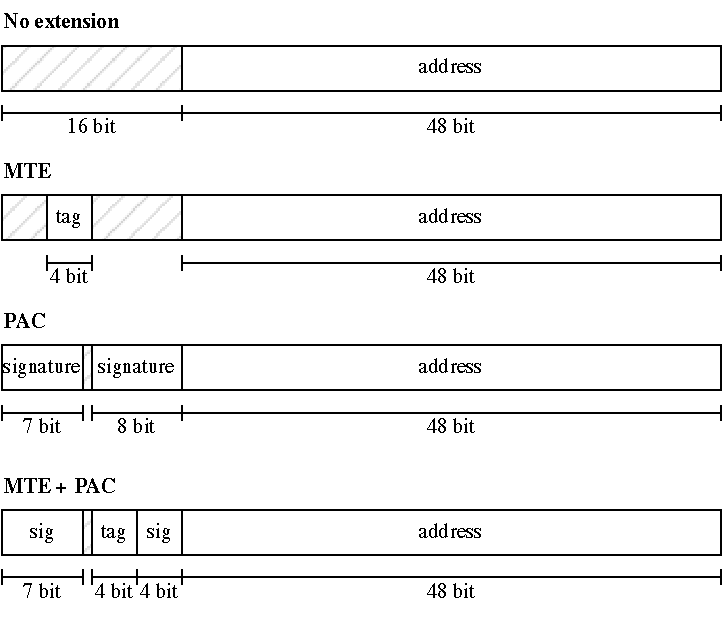
\includegraphics[scale=1]{figures/build/pointer-aarch64}
    \caption{Pointer layout on aarch64 in Linux with and without MTE and PAC enabled}
    \label{fig:aarch64-pointer}
\end{figure}

In \cref{fig:aarch64-pointer}, we show the layout of pointer bits used for address translation in aarch64, the 64\,bit variant of the ArmV8 instruction set\cite{ARMA2024Arch64}, when running on Linux.
Only 48 out of the available 64\ bits are used to address memory, while the remaining bits are set to either 0 or 1 to differentiate between kernel and userspace addresses but are unused for further address translation.
Hardware extensions such as \ac{MTE} (\cref{subsec:mte}) and \ac{PAC} (\cref{subsec:pac}) utilize those unused bits to store metadata.

\subsection{Memory Tagging Extension (MTE)}
\label{subsec:mte}

ARMs \Ac{MTE}, available from ArmV8.5, provides a building block to prevent spatial and temporal memory safety violations~\cite{ARM2019MTE}.
MTE implements a lock-and-key mechanism where memory regions can be tagged with one of 16 distinct tags, and memory access is only allowed using pointers with the corresponding keys.

The locking mechanism is implemented by storing a 4\,bit tag in bits 56--59 of an address (referred to as the logical tag).
Accordingly, a tag is assigned to memory with a granularity of 16\,bytes (referred to as the allocation tag).

On Linux, each process can configure MTE by switching between the following modes:
\begin{itemize}
    \item \textbf{Disabled:} MTE is disabled, and no tag checks are performed.
    \item \textbf{Synchronous:}
    Tag mismatches cause a hardware fault on instruction retirement, a segmentation fault is delivered to the application.
    The faulting instruction cannot read the affected memory location, or the update is not observable in the case of writes.
    \item \textbf{Asynchronous:}
    Tag mismatches do not cause an immediate hardware fault.
    Instructions may be able to read the memory location regardless of tag mismatches, or the update may be observable in the case of writes.
    The fault is delivered after the instruction has retired in the form of a CPU flag.
    The kernel will check this flag at the next context switch and deliver a segmentation fault to the application.
\end{itemize}

\subsection{Pointer Authentication (PAC)}
\label{subsec:pac}

\Ac{PAC}~\cite{Qualcomm2017PointerAuth} introduces primitives to prevent attackers from modifying pointers stored in memory.
The extension provides three instructions for signing pointers, authenticating, or stripping the signature from pointers.
\ac{PAC} places the signature in the upper 16 bits of pointers, with the exact layout dependent on the operating system, hardware, and other factors, such as if \ac{MTE} is enabled.
Signed pointers are invalid and cannot be used to address memory.
They are created using the \texttt{pac*} instructions.
Before being used, the signature needs to be removed.
This happens either with the \texttt{aut*} instructions, which remove the signature if it is valid or produce a pointer that will trap when used if the signature does not match the address.
The extension provides \texttt{strip} instructions to remove the signature regardless of whether it is valid.

\paragraph{} MTE and PAC can be combined at the cost of bits available for the PAC signature.
The exact layout of the PAC signature varies depending on the system.

% TODO: write about LLVM?

% TODO: write about wasmtime/cranelift
